\chapter{性能分析}

在完成第 \ref{chap3} 章中描述性能的性能优化后,将其部署在测试平台下,测试平台由 3 台计算机构成,硬件配置如下所示:

1. 操作系统: Ubuntu 16.04.2 LTS (GNU/Linux 4.4.0-72-generic x86\_64)

2. 中央处理器: Intel(R) Xeon(R) CPU E5-2620 v2 @ 2.10GHz

3. 内存:63149 MB

4. 网卡:Ethernet controller: Broadcom Corporation NetXtreme II BCM57800 1/10 Gigabit Ethernet * 4

5. 硬盘:1.75 TB 机械硬盘

相比第 \ref{chap3} 章中的硬件环境,更多的是计算机之间的物理距离更近,计算机之间的网络延迟更低,更利于分布式平台的搭建。

\section{请求响应时间分析}
Grigorik 等人通过分析大量用户数据,指出用户即使平时生活中接触不到毫秒级别的时间,但是仍能明显感受到毫秒级别的延迟。延迟在 100ms 以内的时候,用户会认为立即得到了响应;在 100 ~ 300 ms 之间,用户会感觉到轻微的延迟;300 ~ 1000 ms 之间,用户仅仅认为系统工作正常,但体验较差;当延迟达到 1000 ms 之上的时候,用户会去做其他工作,不时查看任务是否已经完成;如果延迟达到了 10,000ms 的时候,用户开始怀疑任务程序是否出现了问题,放弃执行任务\upcite{grigorik2013high}。因此,为了满足神经科学家流畅的进行对神经元的实时编辑任务,需要使服务器响应时间控制在 100ms 以内。需要注意的是,用户真正感受到的响应时间还包括前端可视化工作所需的计算时间以及浏览器的渲染时间等,这对服务器的响应时间有了更高的要求。

测试主要针对获如下三类调用量较大的 API 进行测试:

1. 取用户原始图像列表相关 API
2. 用户对神经元结构进行操作的相关 API
3. 获取完整结构脑胞体的响应时间

在这部分的测试中,模拟 100 名用户进行编辑,每名用户的编辑动作进行 3 种操作各 100 个,所有用户共计进行 30,000 次 API 调用。测试结果如图 \ref{response} 所示,响应时间的分布如图 \ref{responsedis} 所示。从图中可以明显的看出绝大多数请求的响应时间集中在 0-20 ms 之间,极少数请求的响应时间超过了 100 ms。按照 Grigorik 分析大量用户数据得出的标准,满足了实时操作的要求。

\begin{figure}
\centering
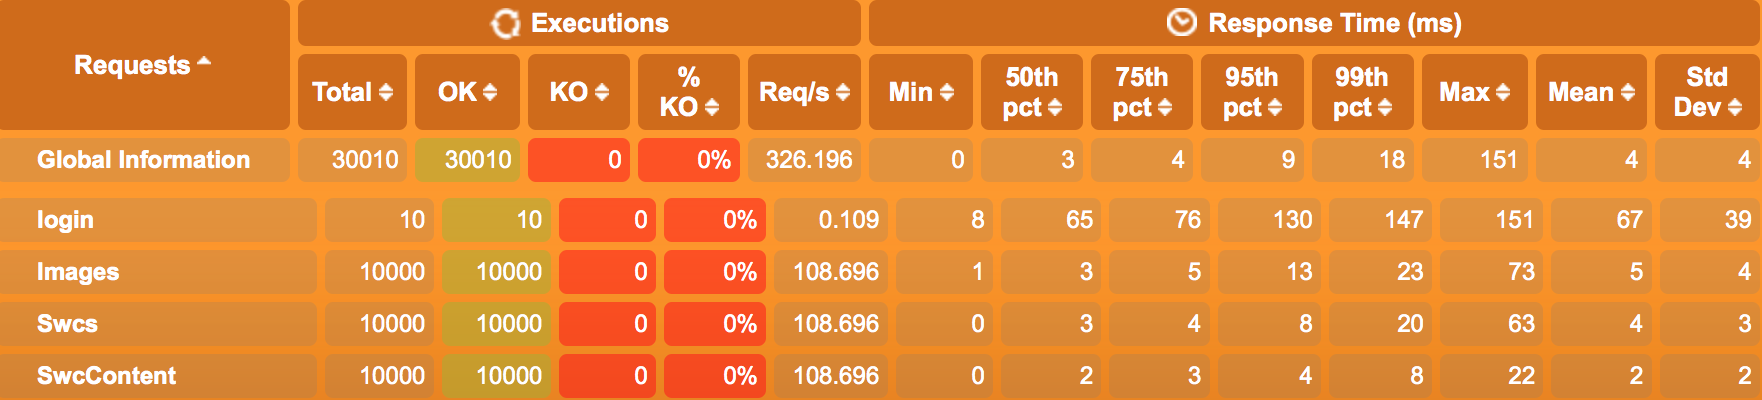
\includegraphics[width=108mm]{images/response}
\caption{请求响应时间,图中 Login 代表用户登录的请求,Images 代表获取用户原始图像列表相关 API 的响应时间,Swcs 代表用户对神经元结构进行操作的相关 API 的响应时间,SwcContent 代表用户获取结构脑胞体的响应时间。}
\label{response}
\end{figure}

\begin{figure}
\centering
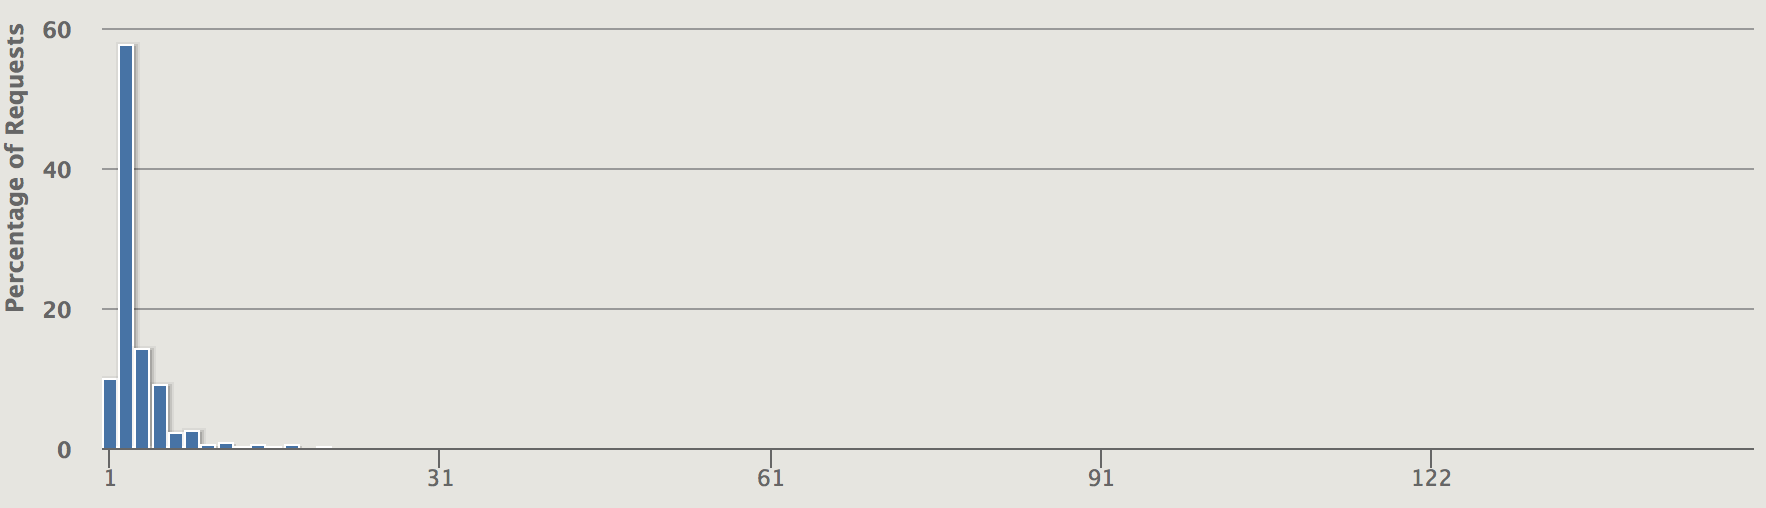
\includegraphics[width=108mm]{images/responsedis}
\caption{所有请求响应时间的分布,可以明显的看出绝大多数请求的响应时间集中在 0-20 ms 之间,极少数请求的响应时间超过了 100 ms。}
\label{responsedis}
\end{figure}

进一步分析响应时间随时间的变化,如图 \ref{responsetime} 所示,可以看出在测试开始时,由于没有缓存,请求的响应时间较高,随着时间的推移,绝大多数的请求被服务器端或者浏览器端缓存下来,响应时间趋于平缓。这说明了使用 Redis 与浏览器端缓存对性能的提升明显,将需要花费一百毫秒才能完成的计算任务降低到可以在毫秒级别内响应,另一方面也降低了服务器的计算压力,使得用户的体验更加流畅。

\begin{figure}
\centering
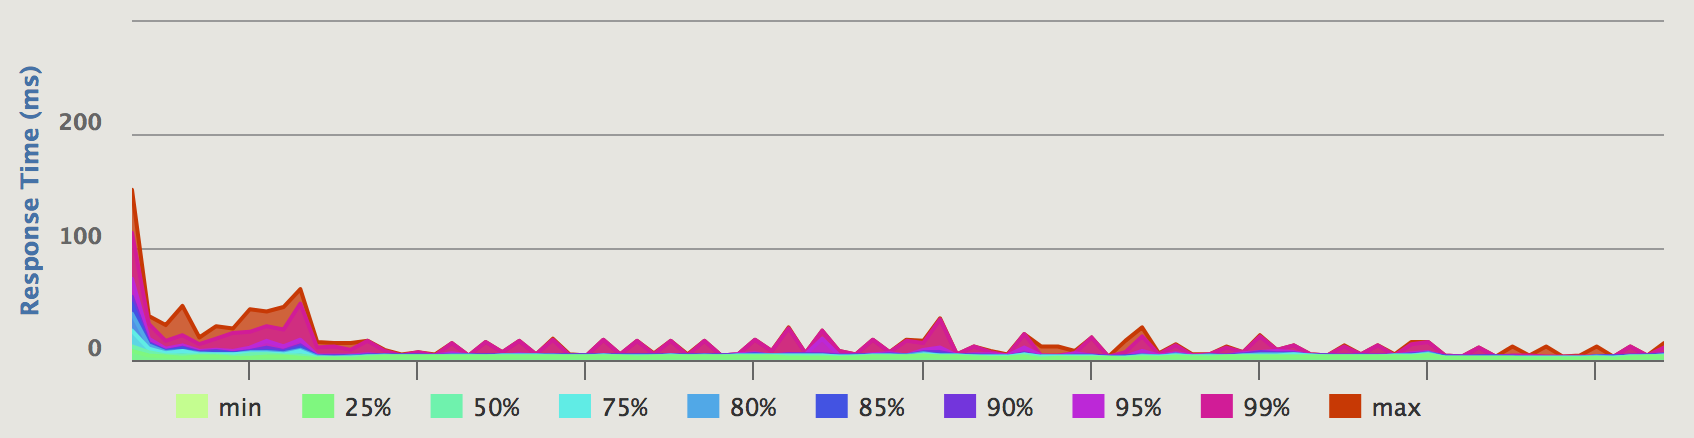
\includegraphics[width=108mm]{images/responsetime}
\caption{请求响应时间随时间的变化,不同颜色标明了不同比例请求所使用的时间。测试开始时,由于没有缓存,请求的响应时间较高,随着时间的推移,绝大多数的请求被服务器端或者浏览器端缓存下来,响应时间趋于平缓。}
\label{responsetime}
\end{figure}

\section{响应请求数量分析}
为了支持多用户同时编辑,平台需要支持多用户同时在线,能够处理大量的并发请求。测试结果如图 \ref{requests},可以看出,经过性能优化之后

\begin{figure}
\centering
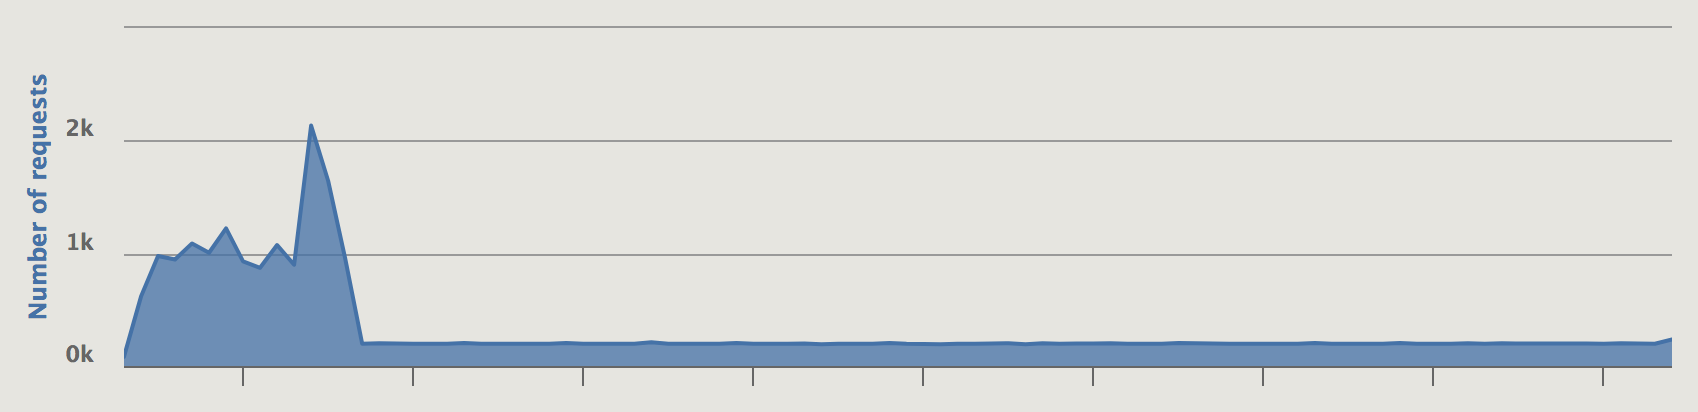
\includegraphics[width=108mm]{images/requests}
\caption{每秒钟响应请求数量}
\label{requests}
\end{figure}

\chapter{总结与展望}
本文设计并实现了一个在线多用户的神经元网络结构编辑分享平台,利用互联网便于数据共享的特点,帮助神经学研究人员便捷地进行异地,多用户协同编辑神经元网络结构,并能分享结构脑图谱,共同探索神经元结构下的奥秘。完成平台搭建后,对平台进行了详细的压力测试,并根据压力测试的结果进行性能调优使之可以支持数千名用户的实时编辑操作。

限于时间关系,平台完成部署后并没有真正投入使用,但是已经与一些神经科学家取得了联系,即将投入神经科学有关结构脑胞体重建和编辑的教学任务中。限于实验室硬件环境尚未完全部署完毕,只有三台计算机可以使用,不能充分发挥分布式结构的优势,在实验室硬件部署完毕后,可以将平台部署在更多的计算机上,充分发挥分布式架构可扩展的特性使之可以支撑更多的用户同时在线。同时结构脑胞体自动重建算法仍然使用的是单机版,脑胞体自动重建算法的并行化已经用 Spark 实现,即将可以在平台中使用,这将进一步提升平台的并行化程度。




